\chapter{Oracle Aplication Express}

\section{Tahapan Membuat Aplikasi Akademik Sederhana Oracle Apex}
Pertama kita membuka gmail dan lihat apakah ada pesan masuk dari oracle-application-express ww@oracle.com selanjutnya , kita akan langsung mempraktekan bagaimana tahapan pembuatan Aplikasi akademik sederhana pada Oracle APEX :

\begin{enumerate}
\item[1] Pergi ke gmail, lihat pesan masuk dari oracle-application-express ww@oracle.com

\begin{figure}[!htbp]
    \begin{center}
    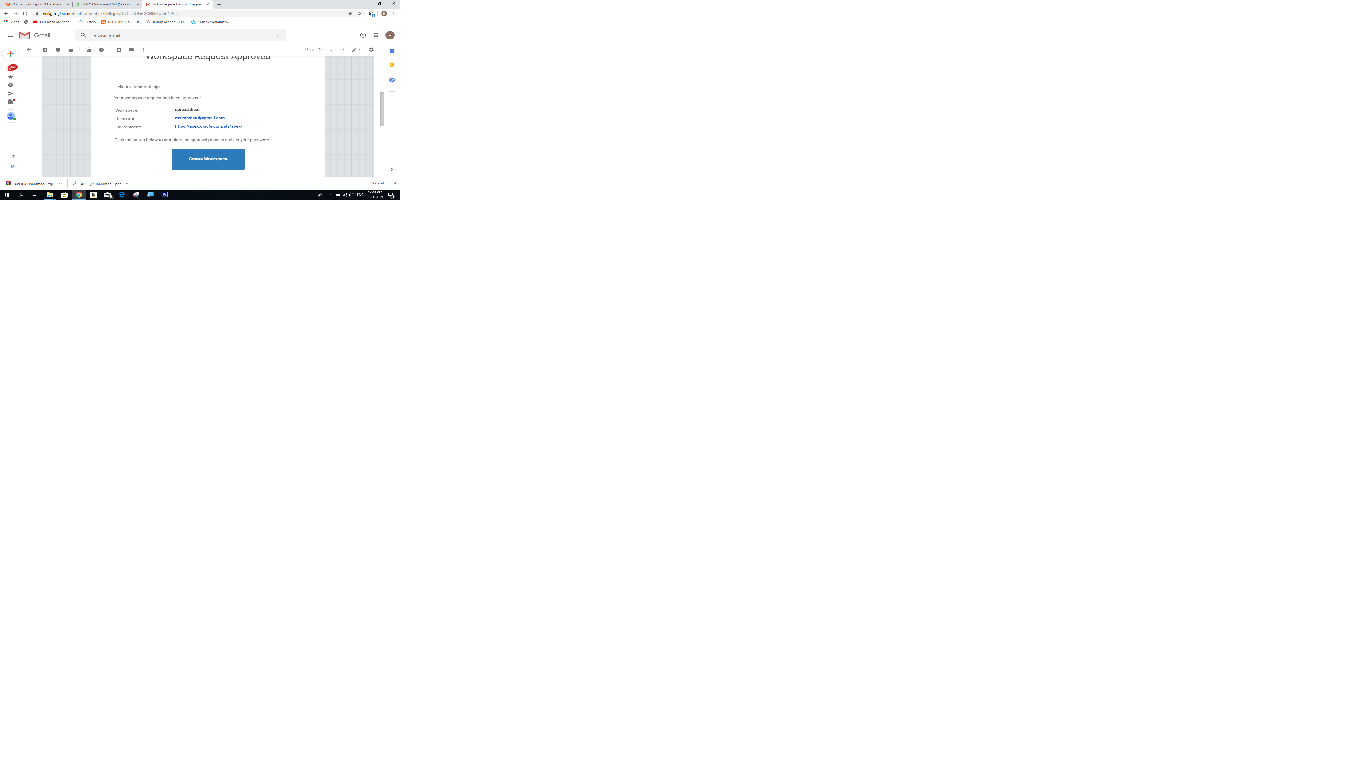
\includegraphics[scale=0.5]{figures/0.png}
    \caption{\textit{Get Start For Free.}}
    \end{center}   
    \end{figure}
    
\begin{figure}[!htbp]
\item[2]Login menggunakan workspace, email dan password yang sudah dibuat sebelumnya.

    \begin{center}
    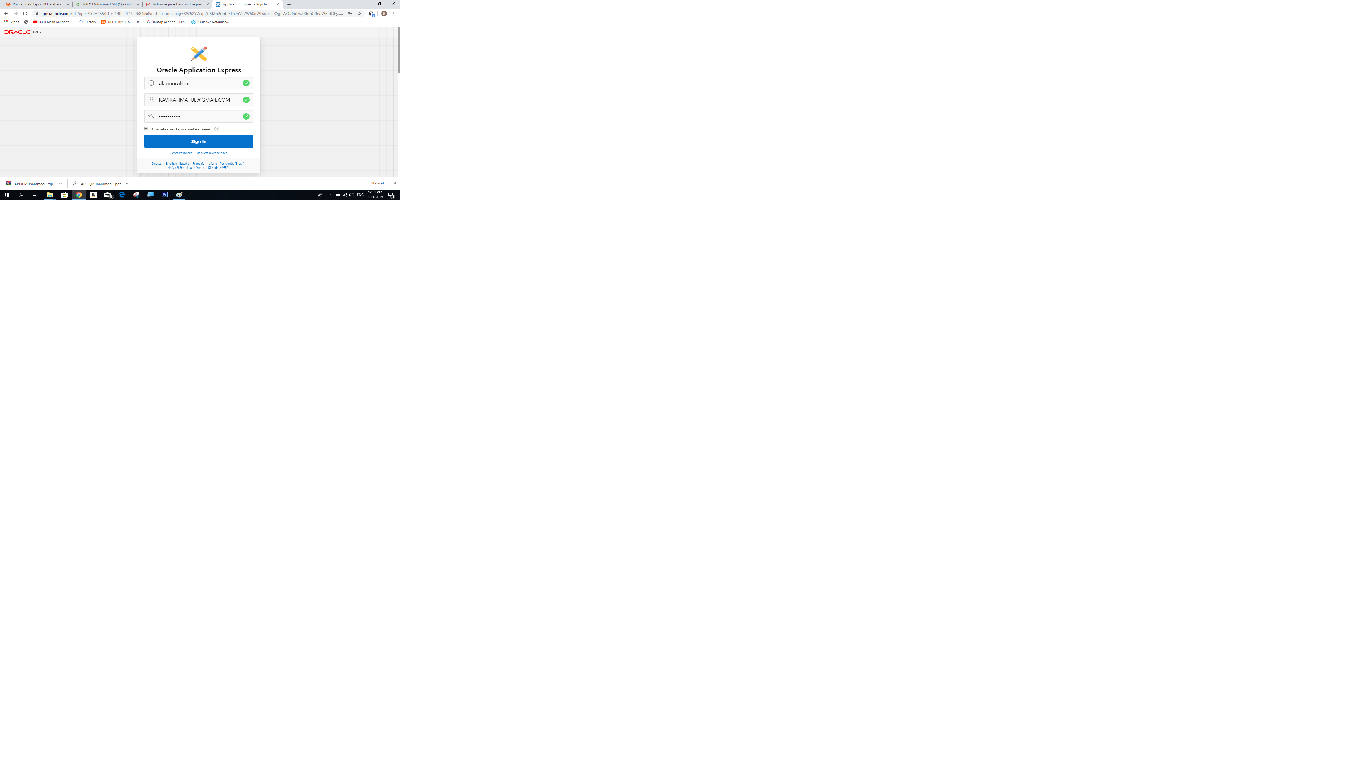
\includegraphics[scale=0.5]{figures/1.png}
    \caption{\textit{Request A Free Workspace.}}
    \end{center}
    \end{figure}
    
\begin{figure}[!htbp]
\item[3]Klik App Builder

    \begin{center}
    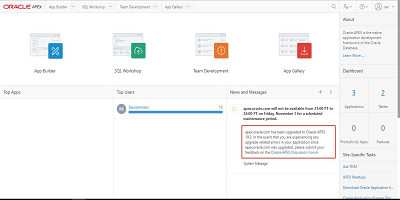
\includegraphics[scale=0.5]{figures/2.png}
    \caption{\textit{Request A Free Workspace.}}
    \end{center}
    \end{figure}
    
\begin{figure}[!htbp]
\item[4]Untuk membuat, Creat app 

    \begin{center}
    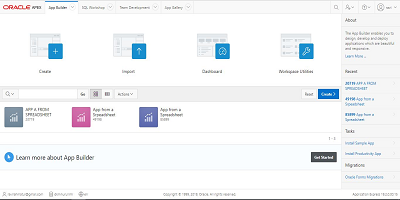
\includegraphics[scale=0.5]{figures/3.png}
    \caption{\textit{Request A Free Workspace.}}
    \end{center}
    \end{figure}

\begin{figure}[!htbp]
\item[5]Klik From a File

    \begin{center}
    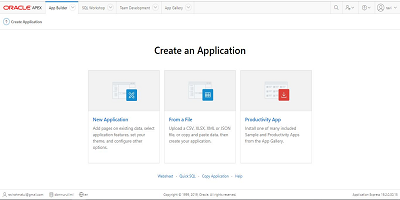
\includegraphics[scale=0.5]{figures/4.png}
    \caption{\textit{Request A Free Workspace.}}
    \end{center}
    \end{figure}
    
\begin{figure}[!htbp]
\item[6]Pilih Filenya

    \begin{center}
    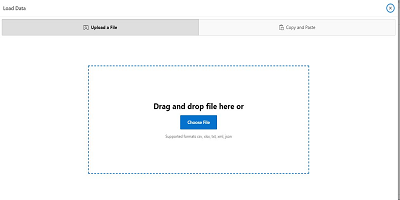
\includegraphics[scale=0.5]{figures/5.png}
    \caption{\textit{Request A Free Workspace.}}
    \end{center}
    \end{figure}

\begin{figure}[!htbp]
\item[7]Klik open

    \begin{center}
    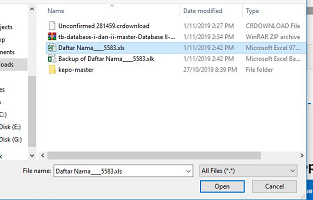
\includegraphics[scale=0.5]{figures/7.png}
    \caption{\textit{Request A Free Workspace.}}
    \end{center}
    \end{figure}

\begin{figure}[!htbp]
\item[8]Klik next

    \begin{center}
    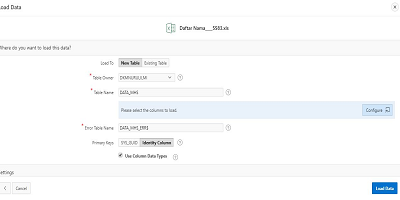
\includegraphics[scale=0.5]{figures/8.png}
    \caption{\textit{Request A Free Workspace.}}
    \end{center}
    \end{figure}

\begin{figure}[!htbp]
\item[9]Klik  select all
    \begin{center}
    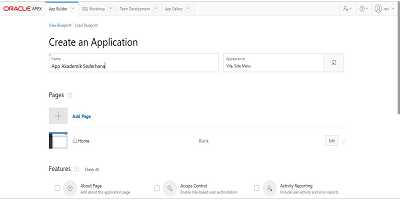
\includegraphics[scale=0.5]{figures/9.png}
    \caption{\textit{Request A Free Workspace.}}
    \end{center}
    \end{figure}
    
\begin{figure}[!htbp]
\item[10]Creat Aplikasi

    \begin{center}
    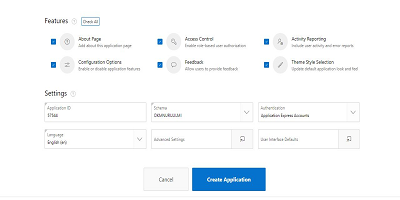
\includegraphics[scale=0.5]{figures/10 .png}
    \caption{\textit{Request A Free Workspace.}}
    \end{center}
    \end{figure}

\begin{figure}[!htbp]
\item[11]Tunggu beberapa saat

    \begin{center}
    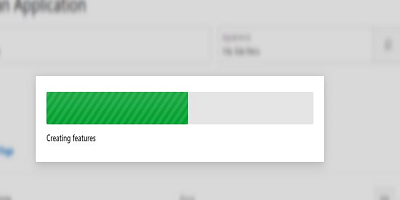
\includegraphics[scale=0.5]{figures/11.png}
    \caption{\textit{Request A Free Workspace.}}
    \end{center}
    \end{figure}

\begin{figure}[!htbp]
\item[12]Klik Run Aplikasi

    \begin{center}
    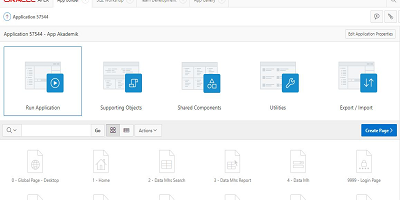
\includegraphics[scale=0.5]{figures/12.png}
    \caption{\textit{Request A Free Workspace.}}
    \end{center}
    \end{figure}

\begin{figure}[!htbp]
\item[13]Lalu Login dengan email dan password yang telah dibuat tadi

    \begin{center}
    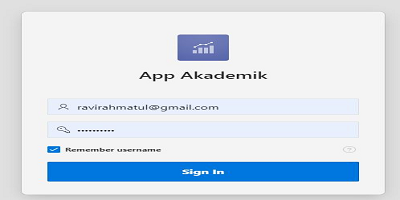
\includegraphics[scale=0.5]{figures/13.png}
    \caption{\textit{Request A Free Workspace.}}
    \end{center}
    \end{figure}

\begin{figure}[!htbp]
\item[14]Aplikasi telah selesai kita buat

    \begin{center}
    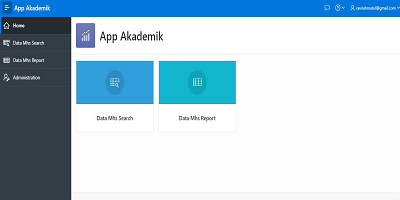
\includegraphics[scale=0.5]{figures/14.png}
    \caption{\textit{Request A Free Workspace.}}
    \end{center}
    \end{figure}
    
\begin{figure}[!htbp]
\item[15]Lihat hasilnya (LINK : https://apex.oracle.com/pls/apex/f?p=57544:1:704747309052112:::::) (Email : ravirahmatul@gmail.com) (Pass: Asus091099)

    \begin{center}
    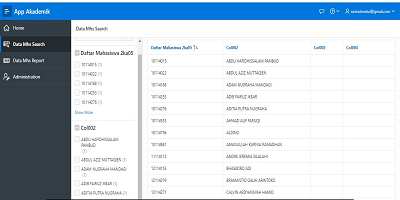
\includegraphics[scale=0.5]{figures/15.png}
    \caption{\textit{Request A Free Workspace.}}
    \end{center}
    \end{figure}


\end{enumerate}
